\section{Generics}

\subsection{Type Constraints}

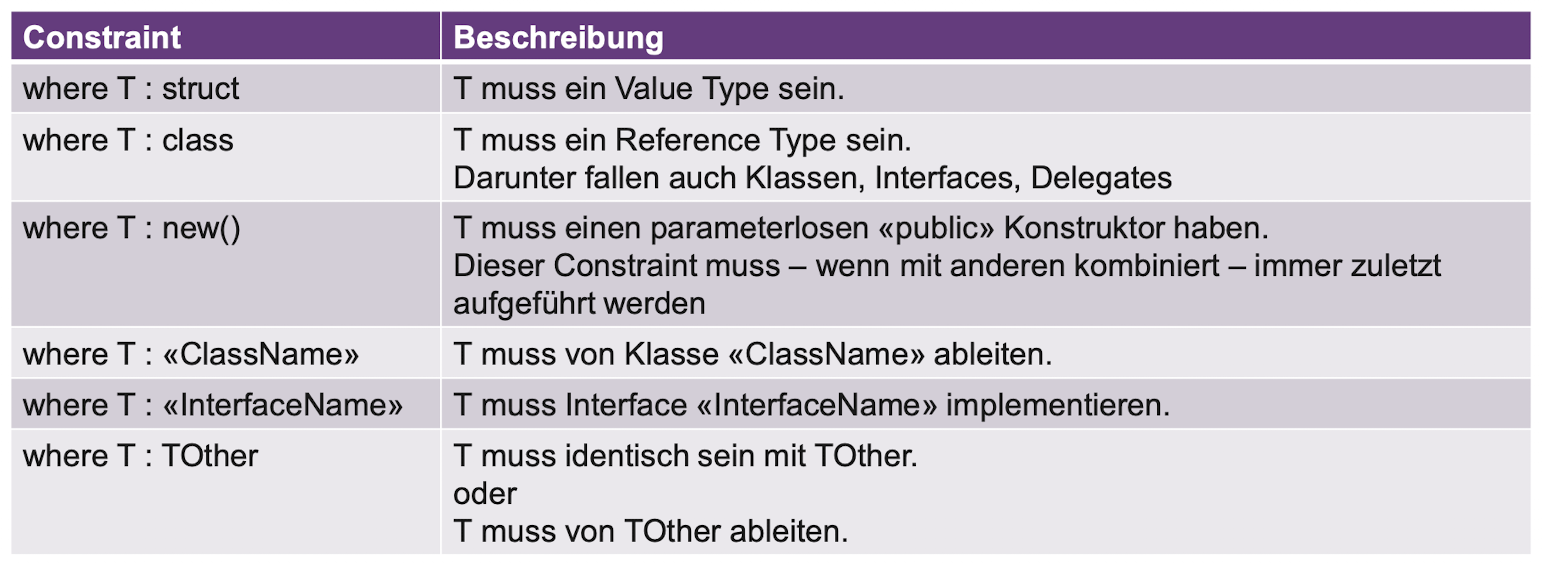
\includegraphics[width=\linewidth]{typeconstraints}

\begin{lstlisting}
static class MyHelpers
    {
        static TDest CopyTo<TSource, TDest, TElement>(TSource source)
        	// Type Constraints for this Operation
            where TSource : IEnumerable<TElement>
            where TDest : IList<TElement>, new()
        {
            TDest dest = new TDest();
            foreach (TElement element in source)
            {
                dest.Add(element);
            }
            return dest;
        }
    }
\end{lstlisting}

\subsection{Type Check}
Prüfungen sind identisch zu den normalen Typen.
\begin{lstlisting}
myVar is Type<T>; // Liefert bool
(Type<T>)myVar; // Liefert Type<T>
myVar as Type<T>;
\end{lstlisting} 

\subsection{Vererbung}
Generische Klassen können von anderen generischen Klassen erben.

\begin{lstlisting}
class MyList<T> : List { }
// Weitergabe des Typparameters an die Basisklasse
class MyList<T> : List<T> { }
// Konkretisierte generische Basisklasse
class MyIntList : List<int> { }
// Mischform
class MyIntKeyDict<T> : Dictionary<int, T> { }
\end{lstlisting}

\subsection{Nullable Types}
Structs können in der Theorie nicht \lstinline{null} sein. \lstinline{default} retourniert den default Wert für den Parametertyp. Vergleiche mit \lstinline{x == null} Refernce Type=true, false, Value Types=false (Compilerfehler wenn Struct).
\begin{lstlisting}
public void NullExamples<T>()
{
	T x1 = null; // Compilerfehler
	T x2 = 0; // Compilerfehler
	T x3 = default(T); // OK 
	T x4 = default; // OK
}
\end{lstlisting}

\subsubsection{Nullable Struct}
Value Types können dank Generics \lstinline{null} zugewiesen werden.
\begin{description}
  \item[HasValue==true] Liefert den Wert, der gespeichert ist
  \item[HasValue==false] \lstinline{System.InvalidOperationException}
\end{description}


\begin{lstlisting}
public struct Nullable<T> where T : struct
{
	public Nullable(T value);
	public Nullable();
	public bool HasValue { get; }
	public T Value { get; }
}
\end{lstlisting}

Danke dem Compiler kann die \lstinline{T?} Syntax verwendet werden. 
\begin{lstlisting}
int? x = 123;
double? y = 1.0;
// Compiler-Output
Nullable<int> x = 123;
Nullable<double> y = 1.0;
// Möglich
x = null; y = null;
int x1 = x.GetValueOrDefault(-1);
int x1 = int(x); // Wenn der Wert Null ist = Problematisch
\end{lstlisting}

\subsubsection{Operatoren (??, ??=)}
\begin{lstlisting}
int i = GetNullableInt() ?? -1;
// Compiler Output
int? iTemp = GetNullableInt();
int i;
if(!iTemp.HasValue) 
{
	i = -1;
} else {
	i = iTemp.GetValueOrDefault();
}
\end{lstlisting}

\begin{lstlisting}
int? i = null;
i ??= 12344; // i = i ?? 1234;
// Compiler-Ouput
int iTemp = i.GetValueOrDefault();
if (!i.HasValue) {
	iTemp = 1234;
	i = iTemp;
}
\end{lstlisting}

\subsubsection{Null Conditional Operator}
Wird eingesetzt für sicheres Method-Chainig, Array-Zugriffe etc.
\begin{lstlisting}
//  Liefert Resultat des rechten Operanden wenn Variable links nicht null ist
string s = GetNullableInt()?.ToString();
\end{lstlisting}

\subsection{Generic Delegate}
Auch Generics unterstützen Delegates.

\begin{lstlisting}
public delegate void Action<T>(T i);
public class MyClass
{
	public static void PrintValue<T>(T i){ 
		Console.WriteLine("Value {0}", i}) 
	}
}
public class FunctionParameterTest
{
	static void ForAll<T>(T[] array, Action<T> a) {
		Console.WriteLine("ForAll called...");
		if(a == null) { return; }
		foreach (T t in array)
		{
			a(t)
		}
}
\end{lstlisting}
